\section{Finding 2: Each Model Implements the Response Its Own Way}
\label{sec:mechanisms}

Shared inputs and shared broad effects leave open whether the models share the \emph{mechanism}: the same
concept, with the same effect, on the same series. At that grain they do not.

\subsection{Fine-grained concepts are organized by model}
\label{sec:bymodel}

The atlas groups causal features from all models whose effect profiles agree at cosine 0.9. It finds more structure than
a column-shuffle null (11 concepts, null 95th percentile 5.05; $p=0.005$), but of the 11 concepts, none spans more than 3
of the 7 models. The clusters are purer by model than random assignment makes them: 9 multi-model concepts against a
null mean of 10.8 ($p_{\text{below}}=0.025$), mean model purity 0.591 against 0.474 (\fid{SH-22}). Five of the 11 are
\emph{convergent}: two models reach the same effect from different series. The result holds held-out: no concept of the
private atlas spans more than 3 of 7 models on v2 or more than 2 on v3 (\fid{SH-16}). Each architecture builds its own
variants of a level or seasonality effect, and several reach the same effect independently.

The clearest component-level example is seasonality. Restoring a deseasonalized context requires one attention head in
TimesFM, but a minimal set of five heads in Chronos-T5-Base whose contributions do not add (path-patching gap 0.0238
against a mean effect of 0.0108; \fid{CA-03}, exploratory). The same capability is a single component in one model and
a nonlinear circuit in another.

\subsection{The same effect on the same series is found only within the Chronos family}
\label{sec:sameeffect}

The strictest test ablates both sides of a reciprocal transfer on the same series. Of 1{,}290 tests, 216 are scorable
(Figure~\ref{fig:funnel}b): 7 show the same causal effect, 54 agree on level or shape alone, 133 show no specific
agreement and 22 act differently. All 7 ``same'' verdicts are between Chronos-2 and Chronos-Bolt, two models from one
family, six of them through one feature set in Chronos-Bolt's fourth block. Because the test never produces a false
``same'' on the planted forecaster, these detections stand. Its insensitivity means that their absence across families
does not prove that effects differ, and the 22 ``acts differently'' verdicts indicate that they sometimes do.
Correspondingly, no registered cross-model causal claim confirms held-out: three multi-model atlas concepts exceed the
null in centroid cosine on private data (0.955--0.988 against 95th percentiles 0.854--0.907) but fail the registered
member-pair rule, and 0 of 6 shared-input agreement claims confirm.

\begin{figure}[!tb]
\centering
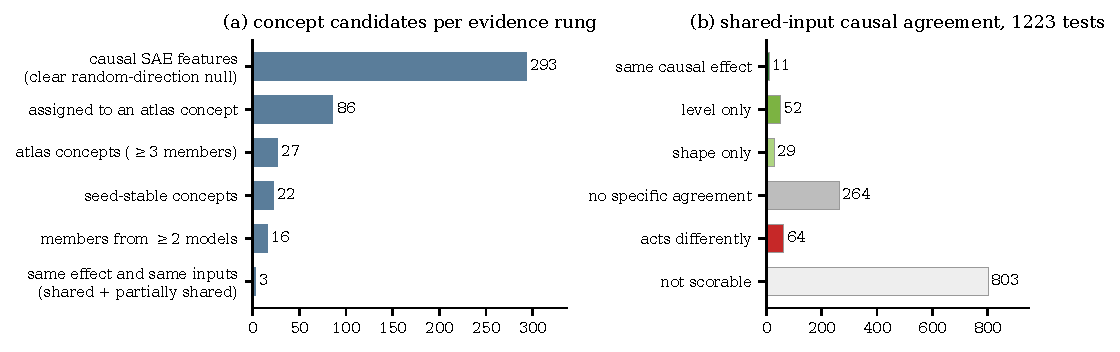
\includegraphics[width=\textwidth]{funnel.pdf}
\caption{(a) Concept candidates at each rung (the first three bars are sequential; the last three are properties of the
11 atlas concepts). (b) Same effect on the same inputs, over 1{,}290 tests drawn from the 1{,}296 reciprocal transfers:
only 7 are ``same'', all within the Chronos family. Source: \texttt{sae/concept\_stage.json}.}
\label{fig:funnel}
\end{figure}

\subsection{Forecast-relevant information is distributed}
\label{sec:distributed}

\paragraph{Causal features exist.} Of 56 target layers, 55 pass both reach controls. Across them, 442 feature-channel
cells clear the isotropic null where the empirical chance rate predicts 178.75 (2.47 times chance), from 1.64 times
(Chronos-T5-Base) to 5.70 (Chronos-Bolt). Timer is the exception: its layers reach the forecast, but its features clear
at 1.02 times chance (\fid{PM-17}). Target by target, 22 of 55 targets clear significantly more cells than chance, at
least two in every model except Timer. Registered single-feature effects replicate in part: 10 of 31 testable claims
confirm on the v2 private split, each at the Holm floor for 31 tests ($p_{\text{Holm}}=0.031$), and 11 of 24 on v3.

\paragraph{But single features are only weakly special.} The v3 run scored every feature against both nulls. Under the
isotropic null, 238 of 967 scorable features clear at least one channel; under the covariance-matched null, 91 do.
Scoring each null draw as a pseudo-feature on all nine channels at once gives expected counts of 67.0 and 70.4, so
features exceed chance 3.55-fold against isotropic directions ($p=4\times10^{-86}$) but only 1.29-fold against directions
drawn from the activation distribution ($p=0.0045$). Removing a typical on-manifold direction moves the forecast nearly
as much as removing a dictionary feature. The effects are also small: the median single-feature effect is 0.097 context
standard deviations, 2.2 times smaller than the 0.214 by which substituting the reconstruction moves the forecast (v3:
1.7 times; \fid{MN-15}).

\paragraph{Effects persist under other interventions, but the clearing set shifts.} We re-tested the 91 v3 features
that clear the on-manifold null under three on-manifold interventions, each with its own matched null: replacing the
feature by its corpus mean, by its activation on another series where it fires, or subtracting it from the model's own
activation rather than the reconstruction. 79 of 91 clear under at least one and 37 under all three; mean and resample
ablation keep the direction of the effect (median cosine to zero ablation 0.997 and 0.991; \fid{MP-10}). Most causal
features have a real effect, but which ones clear depends on the intervention.

\paragraph{Effects form a continuum, not discrete units.} Within a layer, 50 of 56 targets are non-modular: no
choice of $k$ splits their effect vectors into clusters of at least three members each. The families of
Section~\ref{sec:families} cover 192 of 194 features but do not beat a column-shuffle null in number ($p=0.68$), and the
silhouette is 0.25--0.32 for every cut from 6 to 16 families. The effect vectors are not low-dimensional (participation
ratio 5.58 of 9 channels on v3; \fid{MN-07}), so the absence of discrete units is not a lack of variation. Combined with
the on-manifold result, the picture is of forecast-relevant information spread across many directions, graded rather
than modular. This is a different picture from the monosemantic units sought in language models
\citep{bricken2023monosemanticity}, and it implies that a single-feature claim about a TSFM should be stated against an
on-manifold null.
